\documentclass{beamer}

\usetheme{Madrid}
\usecolortheme{beaver}

\usepackage{amsmath}
\usepackage{amssymb}
\usepackage{graphicx}
\usepackage{subcaption}
\usepackage{bbm}
\usepackage{booktabs}
\usepackage{url}
\usepackage{cancel}

\usepackage[style=authoryear, fontsize=11]{biblatex}
\addbibresource{references.bib}

\renewcommand{\footnotesize}{\tiny}

\title[Power law attention biases]{Power law attention biases for molecular transformers}
\author{Jay Shen}

\begin{document}

% -------------------------------------------------------
\begin{frame}
    \titlepage
\end{frame}
% -------------------------------------------------------

\begin{frame}{Motivation}
    Transformers scale well and are dominant in most domains, but are rarely used for electronic structure prediction over equivariant GNNs\footcite{li-mlip-review}\footcite{jacobs-mlip-review}.

    \vspace{1em}
    
    Is this due to a lack of good inductive biases for many-body geometry?
    
    $\rightarrow$ If so, how can we design better ones? 

\end{frame}

% -------------------------------------------------------
\section{Background}

\begin{frame}{The problem with dot-product attention}

The vanilla attention mechanism has the form:
\[
A_{ij}=\mathrm{softmax}_j\left( \frac{q_i k_j^T}{\sqrt{d_k}} \right)
\]
The implication is that a token's embedding must also encode its relationships to other tokens—typically, this is accomplished using positional encodings. 
\begin{itemize}
    \item This is fine for modalities like language and image, which admit absolute positional indices. 
    \item But it is bad for modalities, like graphs and point clouds, with implicit degeneracies (rotation, translation, permutation). 
\end{itemize}
\end{frame}

\begin{frame}{Biased attention}

Attention biases model global structure without positional encodings by adding values $b_{ij}$ to pre-softmax attention logits. 
\[
A_{ij}=\mathrm{softmax}_j\left( \frac{q_i k_j^T}{\sqrt{d_k}} + b_{ij} \right)
\]
One conceptual advantage is that attention biases are naturally \textit{pairwise}, just like the laws of physics! Think about Newton's law of gravitation, for instance. 

\vspace{1em}

As we will see, attention biases can be naturally constructed given a measure of \textit{distance} between two tokens \footcite{swin}. 

\end{frame}

% -------------------------------------------------------
\section{Power Law Attention Biases}

\begin{frame}{Power law attention biases}

Consider the $E(3)$ equivariant bias $b_{ij}=p \log ||\mathbf{r}_i - \mathbf{r}_j||$. 

\vspace{1em}

When passed through the softmax function:
\begin{equation*}
\begin{split}
    A_{ij} &= \text{softmax}_j \biggr [\frac{\mathbf{q}_{i} \mathbf{k}_j^T}{\sqrt{d_k}} + p \log || \mathbf{r}_i - \mathbf{r}_j || \biggr] \\
    &\propto \exp \biggr[ \frac{\mathbf{q}_{i} \mathbf{k}_j^T}{\sqrt{d_k}} + p \log || \mathbf{r}_i - \mathbf{r}_j || \biggr] \\
    &= || \mathbf{r}_i - \mathbf{r}_j ||^{p}\exp \biggr[ \frac{\mathbf{q}_{i} \mathbf{k}_j^T}{\sqrt{d_k}} \biggr]
\end{split}
\end{equation*}
So the bias \textit{weights} attention by a power of the interatomic distance. 

\vspace{1em}

This is analogous to physical interactions such as Coulomb's law, where the interaction strength is modulated by distance as well as the charges/embeddings of the particles/tokens. 

\end{frame}

\begin{frame}{Power law attention biases in practice}

We have quite a bit of design freedom when it comes to selecting $p$. We can:
\begin{itemize}
    \item Learn an exponent $p \in \mathbb{R}$. 
    \item Learn a strictly negative exponent $p \in \mathbb{R}_-$ by reparameterizing $p=-e^\theta$. 
    \item Fix $p$, for example as $p = -1$ (potential energy fall off from physics)
\end{itemize}
We can also use different exponents $p$ per attention head per layer, which should increase model expressivity. 

\end{frame}

% -------------------------------------------------------
\section{Experiments}

\begin{frame}{Experiments}

We test this approach against a few other inductive biases (positional encodings, graph attention) using a standardized transformer architecture and training procedure:
\begin{table}
    \scriptsize
    \centering
    \begin{tabular}{lc}
    \toprule
    Embedding dimension & 128 \\
    Number of layers & 8 \\
    Number of attention heads & 8 \\
    Dropout & 0.1 \\
    Number of epochs & 128 \\
    Batch size & 64 \\
    Learning rate & 0.0001 \\
    Weight Decay & 0.00001 \\
    \bottomrule
    \end{tabular}
\end{table}

We benchmark on electronic structure prediction tasks:
\begin{itemize}
    \item QM9: orbital energies HOMO, LUMO and state energies $U$, $H$, $G$
    \item SPICE: formation energy $U_F$
\end{itemize}

\end{frame}

\begin{frame}{Results}
\begin{table}[ht]
    \scriptsize
    \centering
    \begin{tabular}{l c ccccc c c}
        \noalign{\vskip 1em}
        \toprule
        &&\multicolumn{5}{c}{QM9} && \multicolumn{1}{c}{SPICE} \\
        \cline{3-7}\cline{9-9}
        \noalign{\vskip 2pt}
        Structural bias && HOMO & LUMO & $U$ & $H$ & $G$ && $U_F$\\
        \hline
        \noalign{\vskip 2pt}
        
        Transformer && 0.34 & 0.74 & 24 & 24 & 24 && 10 \\
        Graph Attention && 0.12 & 0.14 & 29 & 29 & 30 && - \\
        RWPE && 0.14 & 0.20 & 42 & 42 & 42 && - \\
        \noalign{\vskip 2pt}
        Attention bias && & & & & && \\
        \cline{0-0}
        \noalign{\vskip 2pt}
        Gaussian kernel && 0.08 & 0.10 & 21 & 21 & 21 && - \\
        Power law $p=-1$ && 0.11 & 0.13 & 26 & 26 & 26 && 7 \\
        Power law $p \in \mathbb{R}$ && 0.12 & 0.14 & 25 & 25 & 25 && 5 \\
        Power law $p\in \mathbb{R}_-$ && 0.11 & 0.12 & 21 & 21 & 21 && 5 \\
        \bottomrule
    \end{tabular}
    \caption{Test ensemble mean absolute errors (eV)}
\end{table}

Experiments suggest: 
\begin{itemize}
    \item Attention biases generally outperform other inductive biases. 
    \item Learned inverse power law biases ($p\in \mathbb{R}_-$) are competitive with the more complex Gaussian kernel biases\footcite{gaussian-kernel}. 
\end{itemize}

\end{frame}

\begin{frame}{Learned exponents}
\begin{figure}[ht]
    \centering
    \begin{subfigure}[t]{0.25\textwidth}
        \centering
        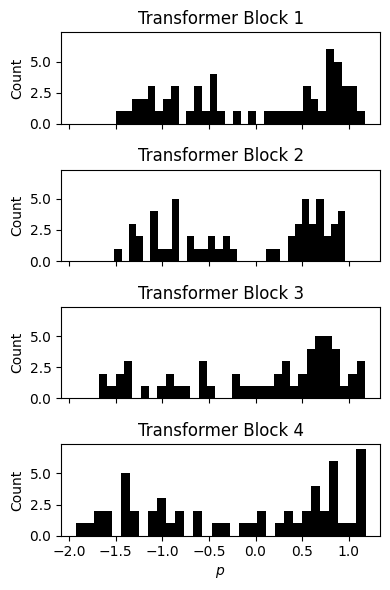
\includegraphics[width=\linewidth]{figures/exponents_unconstrained.png}
        \caption{$p\in\mathbb{R}$}
    \end{subfigure}%
    \hspace{2.5em}
    \begin{subfigure}[t]{0.25\textwidth}
        \centering
        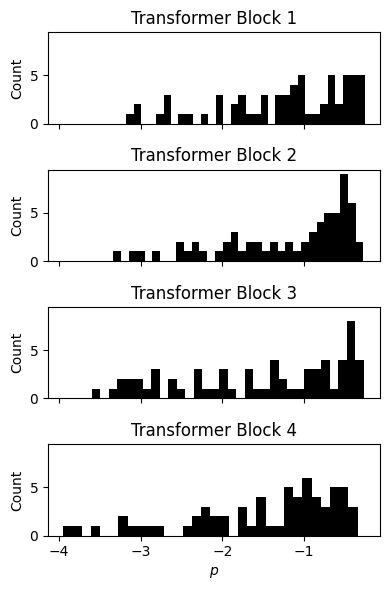
\includegraphics[width=\linewidth]{figures/exponents_negative.png}
        \caption{$p\in\mathbb{R}^-$}
    \end{subfigure}
    \caption{Histogram of learned power law exponents.}
\end{figure}

Unfortunately, learned exponents don't seem to be interpretable and, when unconstrained, are sometimes $>0$ (unphysical). 

\end{frame}

% -------------------------------------------------------
\section{Ablation Study}

\begin{frame}{Ablating dot-product attention}

Experiments show attention biases outperform other inductive biases, but:
\begin{enumerate}
    \item How much modeling capacity do attention biases have by themselves?
    \item Can we use them as substitutes for dot-product attention entirely? 
\end{enumerate}
We test this by ablating dot-product attention:
\[
A_{ij}=\mathrm{softmax}_j\left(\: \cancel{\frac{q_i k_j^T}{\sqrt{d_k}}}  + b_{ij} \right) \quad \rightarrow \quad A_{ij} = \mathrm{softmax}_j(b_{ij})
\]
In this form, attention $\equiv$ weighted message passing on a complete graph!  
\end{frame}

\begin{frame}{Effect of ablation}
\begin{table}[ht]
    \scriptsize
    \centering
    \begin{tabular}{l c ccccc}
        \noalign{\vskip 1em}
        \toprule
         && HOMO & LUMO & $U$ & $H$ & $G$ \\
        \hline
        \noalign{\vskip 2pt}
        Transformer && 0.34 & 0.74 & 24 & 24 & 24 \\
        \noalign{\vskip 2pt}
        Attention bias &&&&&& \\
        \cline{0-0}
        \noalign{\vskip 2pt}
        Gaussian kernel && 0.1 (+8\%) & 0.1 (+7\%) & 20 (-5\%) & 20 (-6\%) & 20 (-7\%) \\
        Power law $p=-1$ && 0.1 (+14\%) & 0.2 (+19\%) & 27 (+3\%) & 27 (+2\%) & 27 (+4\%) \\
        Power law $p\in \mathbb{R}$ && 0.1 (+9\%) & 0.1 (+11\%) & 26 (+3\%) & 25 (+2\%) & 25 (+3\%) \\
        Power law $p \in \mathbb{R}_-$ && 0.1 (+11\%) & 0.1 (+12\%) & 25 (+9\%) & 25 (+8\%) & 25 (+9\%) \\
        \bottomrule
    \end{tabular}
    \caption{Ensemble mean MAE (eV) of ablated models. Percent change from unablated MAE in parentheses. }
\end{table}

\begin{itemize}
    \item Percent change is generally not huge! Ablated models better than vanilla Transformer on HOMO, LUMO
    \item{
        In the case of Gaussian kernel biases, performance actually improves. 
        \begin{itemize}
            \item Gaussian kernel biases are fairly complex, which explains why they are able to compensate so well. 
        \end{itemize}
    }
\end{itemize}

\end{frame}

\begin{frame}{Learned exponents of ablated models}
\begin{figure}[ht]
    \centering
    \begin{subfigure}[t]{0.25\textwidth}
        \centering
        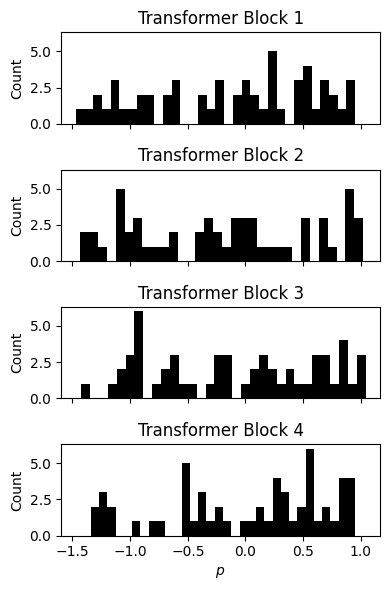
\includegraphics[width=\linewidth]{figures/exponents_unconstrained_fixed.png}
        \caption{$p\in\mathbb{R}$}
    \end{subfigure}%
    \hspace{2.5em}
    \begin{subfigure}[t]{0.25\textwidth}
        \centering
        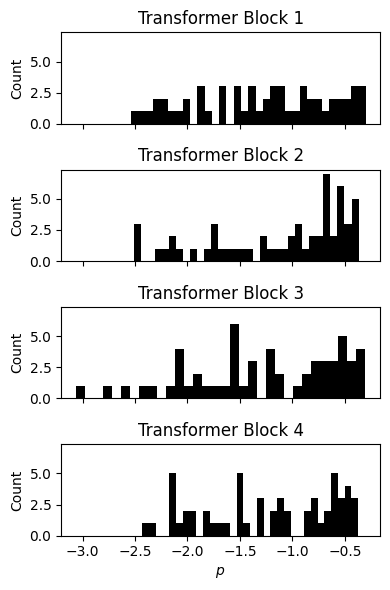
\includegraphics[width=\linewidth]{figures/exponents_negative_fixed.png}
        \caption{$p\in\mathbb{R}^-$}
    \end{subfigure}
    \caption{Histogram of learned power law exponents when dot-product attention is ablated. }
    \label{fig:exponents_fixed}
\end{figure}

Learned power law exponents, when dot-product attention is ablated, are still uninterpretable. 

\end{frame}

% -------------------------------------------------------
\section{Conclusions}

\begin{frame}{Conclusions}
    We conclude power law attention biases are:
    \begin{itemize}
        \item Simple, physically motivated, and more effective than positional encodings and graph attention. 
        \item Uninterpretable, unfortunately :(
        \item Competitive with Gaussian kernels at much lower computational cost. 
    \end{itemize}
    We also note that good attention biases can cheaply compensate for the ablation of dot-product attention. 

    \vspace{1em}
    
    In the future:
    \begin{itemize}
        \item Reevaluate at different scales (model/data/compute). 
        \item {
            Explore design space at depth. 
            \begin{itemize}
                \item For example, are there initializations which induce more interpretable exponents? 
            \end{itemize}
        }
    \end{itemize}
\end{frame}

\begin{frame}{Related works}



\begin{figure}[ht]
    \centering
    \begin{subfigure}[t]{0.45\textwidth}
        \centering
        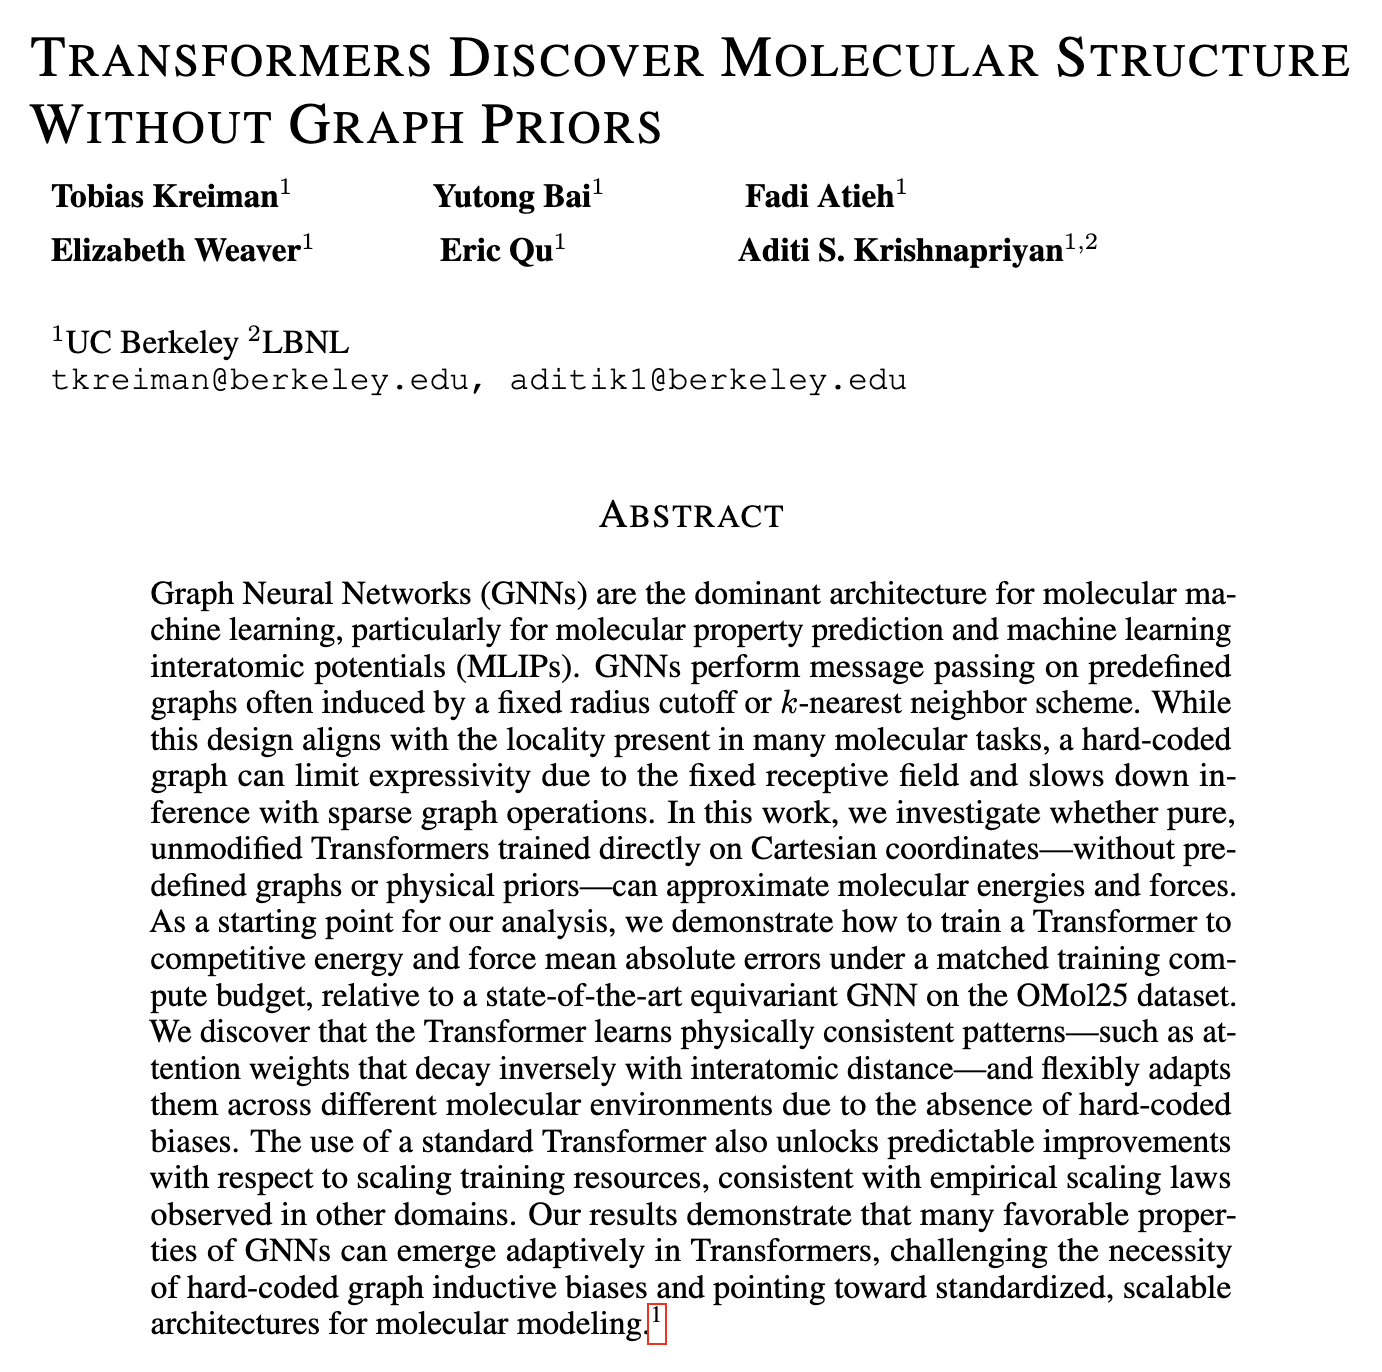
\includegraphics[width=\linewidth]{figures/kreiman_etal.png}
        \caption{\url{https://arxiv.org/abs/2510.02259}}
    \end{subfigure}%
    \hspace{2.5em}
    \begin{subfigure}[t]{0.45\textwidth}
        \centering
        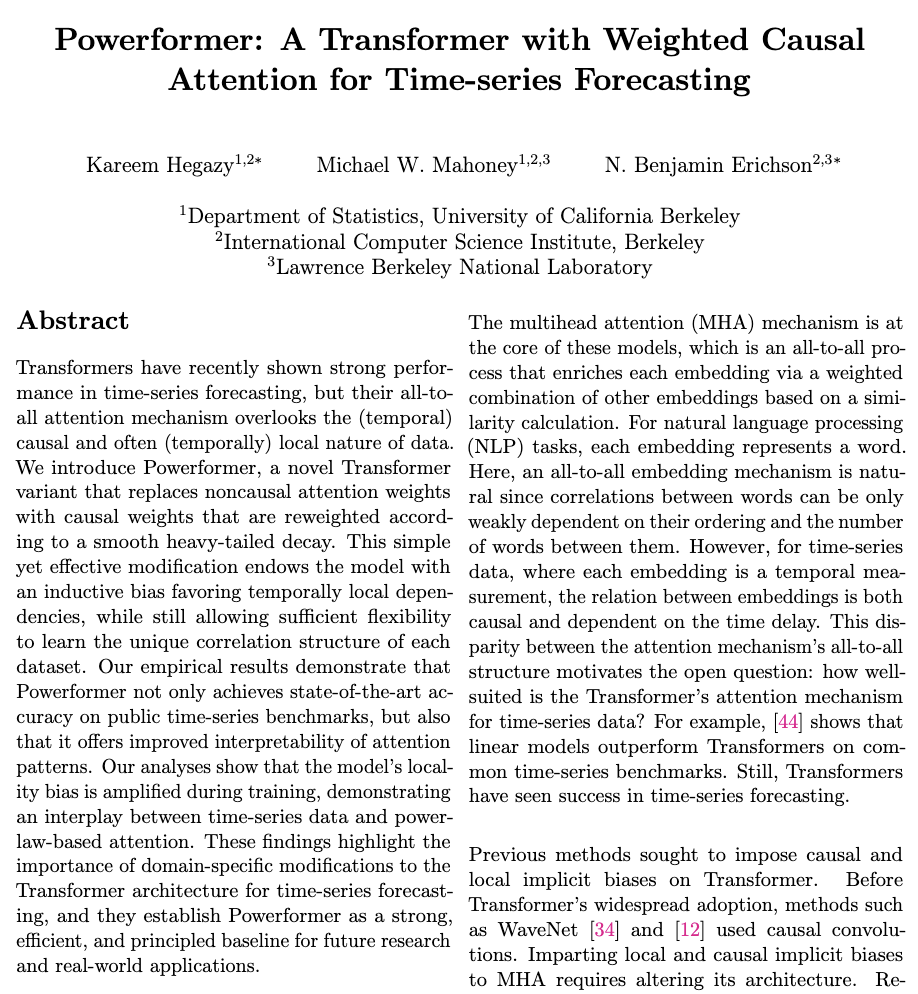
\includegraphics[width=\linewidth]{figures/hegazy_etal.png}
        \caption{\url{https://arxiv.org/pdf/2502.06151}}
    \end{subfigure}
\end{figure}

\end{frame}

\begin{frame}{Thanks! Questions? }
\centering
\small
Code: \url{https://github.com/jshe2304/molecular_attention_bias}

Paper: \url{https://arxiv.org/abs/2511.11489}
\end{frame}

\end{document}
